\documentclass[12pt]{article}

\usepackage[utf8]{inputenc}
\usepackage[brazil]{babel}
\usepackage[a4paper,left=3cm, right=2cm,top=2.5cm, bottom=2.5cm]{geometry}
\usepackage{amsmath}
\usepackage{graphicx}
\usepackage{float}
\usepackage{multirow}
\usepackage{authblk}
\usepackage{fancyhdr}
\usepackage{xcolor}
\usepackage{cite}


\title{\textbf{ENG1456 - Lógica Fuzzy - Trabalho 2}}
\author{\textbf{Aluno: Matheus Carneiro Nogueira - 1810764}}
\affil{}
\author{\textbf{Professora: Ricardo Tanscheit}}
\affil{}
\pagestyle{fancy}
\fancyhf{}
\lhead{{\small \textcolor{gray}{PUC-Rio ENG1456}}}
\renewcommand{\headrulewidth}{0pt}
\date{}
\renewcommand{\footrulewidth}{0pt}
\fancyfoot[C]{\thepage}

\begin{document}
	\maketitle
	\tableofcontents
	

\begin{abstract}
	Este documento consiste no relatório do trabalho 2 do módulo de Lógica Fuzzy da disciplina ENG1456 da PUC-Rio. O trabalho é dividido em duas partes. Primeiramente, o objetivo é alterar o banco de regras em duas situações distintas com o intuito de fazer o container ser parar no local correto. A segunda parte consiste em calcular manualmente as saídas de cada base de regras e a resposta final do sistema de inferência para as variáveis definidas no problema imobiliário. Será utilizado o software Fuzzytech para a realização deste trabalho.
\end{abstract}

\section{Parte 1 - Controle do Guindaste}

\subsection{QR 1 - Exibindo estado inicial}

Antes de alterar o banco de regras do sistema de controle fuzzy para o controle do guindaste, as figuras abaixo exibem o estado inicial dessas regras. Além disso, também é exibida uma figura que mostra a posição final do container na situação 1.
\begin{figure}[H]
	\centering
	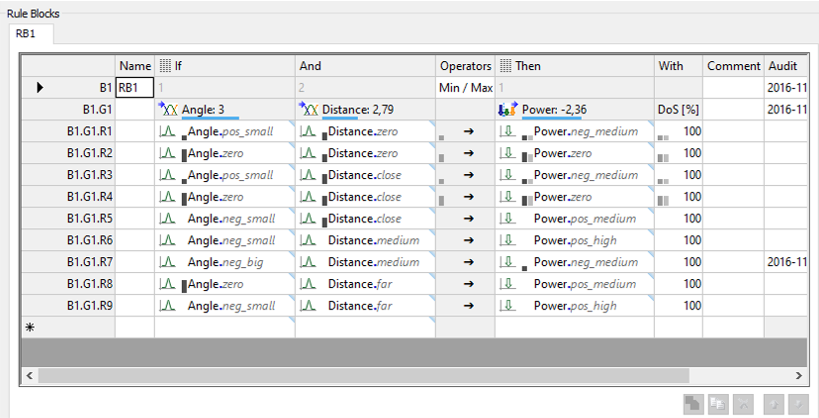
\includegraphics[width=0.9\linewidth]{Imagens/QR1/regrasOriginais}
	\caption{Regras originais}
	\label{fig:regrasoriginais}
\end{figure}
\begin{figure}[H]
	\centering
	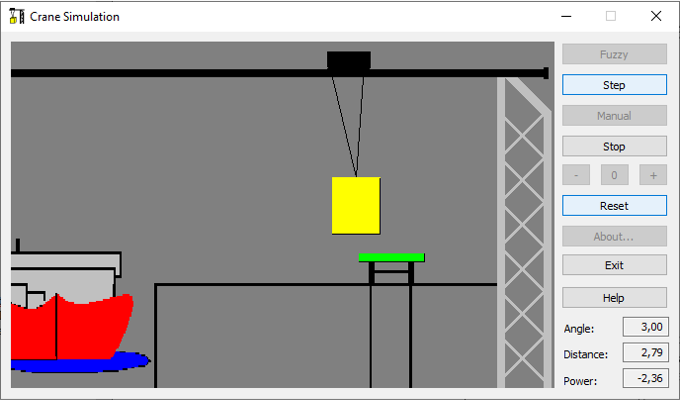
\includegraphics[width=0.9\linewidth]{Imagens/QR1/posicaoFinalOriginal}
	\caption{Posição Final original do container}
	\label{fig:posicaoFinalOriginal}
\end{figure}

A partir da figura \ref{fig:posicaoFinalOriginal} pode-se perceber que o guindaste parou antes da posição correta. Vale a pena, antes de mudar as regras arbitrariamente,  analisar as regras originais para tentar encontrar alguma regra mal definida.

Primeiramente, nota-se que existem duas regras cuja consequência é \textit{Power.zero}. São elas:
\begin{align*}
	Angle.zero\&Distance.zero\to Power.zero\\
	Angle.zero\&Distance.close\to Power.zero
\end{align*}

A primeira regra faz sentido, uma vez que os dois antecedentes indicam que o guindaste chegou na posição correta, o que implica que ele deve ser desligado. A segunda, por outro lado, é estranha. Ao se aproximar do local destino, isto é, à medida que a distância fica próxima, é natural que queiramos diminuir a potência do guindaste, mas não zerá-la completamente. Essa será a primeira regra a ser alterada.

\subsection{QR 1 - Alteração de Regras}

Como comentado, a primeira alteração a ser feita é alterar a regra $(1)$ abaixo. Como o guindaste parou um pouco antes do local adequado, alteremos essa regra para $(2)$, pois queremos que o guindaste ainda ande um pouco para a direita.

\begin{align}
	Angle.zero\&Distance.close&\to Power.zero\\
	Angle.zero\&Distance.close&\to Power.pos\_medium
\end{align}

O resultado dessa alteração é exibido na figura abaixo.
\begin{figure}[H]
	\centering
	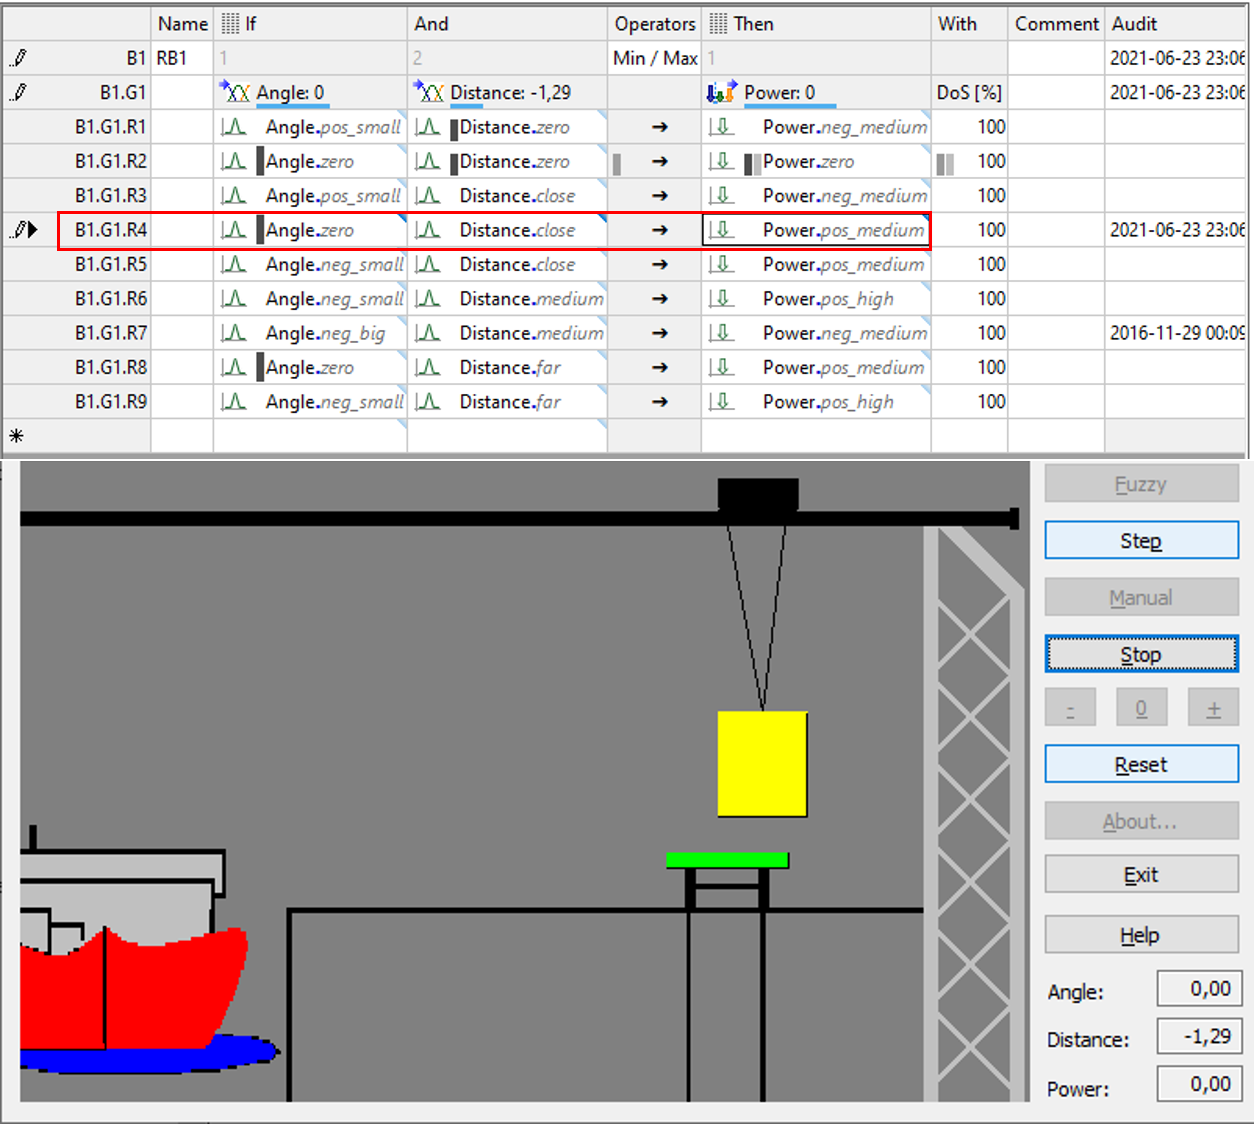
\includegraphics[width=0.7\linewidth]{Imagens/QR1/alteracao1}
	\caption{Resultado da primeira alteração}
	\label{fig:alteracao1}
\end{figure}

Com isso, o guindaste passou um pouco do local final adequado. Podemos tentar contrabalancear isso alterando a regra $(3)$ abaixo para $(4)$. 

\begin{align}
	Angle.pos\_small\&Distance.close&\to Power.neg\_medium\\
	Angle.pos\_small\&Distance.close&\to Power.neg\_high
\end{align}

O resultado encontra-se abaixo.
\begin{figure}[H]
	\centering
	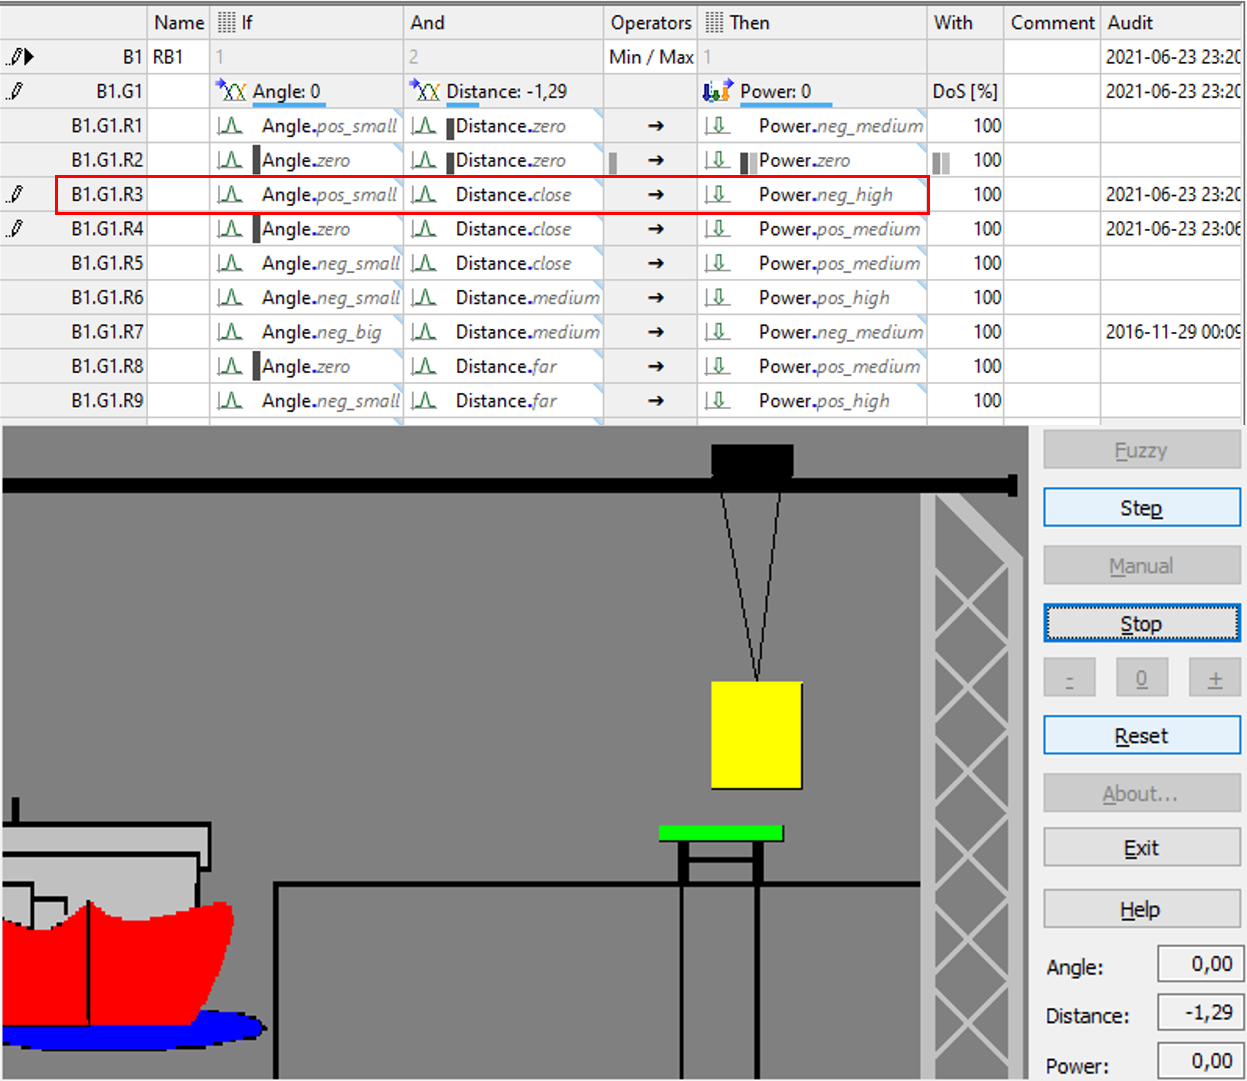
\includegraphics[width=0.7\linewidth]{Imagens/QR1/alteracao2}
	\caption{Resultado da segunda alteração}
	\label{fig:alteracao2}
\end{figure}

Pouca diferença é notada após essa segunda alteração. Sendo assim, ainda é necessária uma alteração que ou impeça o guindaste de passar da posição correta ou que, uma vez ultrapassada, faça o guindaste retornar. Como não existe na variável \textit{Distance} um valor que expresse a ultrapassagem. O enunciado estabelece que é proibida a exclusão de regras, mas não diz nada sobre a inclusão de novas regras. Sendo assim, foi incluída a regra $(5)$ abaixo para fazer com que o guindaste, se passar do local correto, volte um pouco.
\begin{equation}
	Angle.zero\&Distance.neg\_close\to Power.neg\_medium
\end{equation}

A figura abaixo exibe o resultado obtido com a inclusão dessa regra.

\begin{figure}[H]
	\centering
	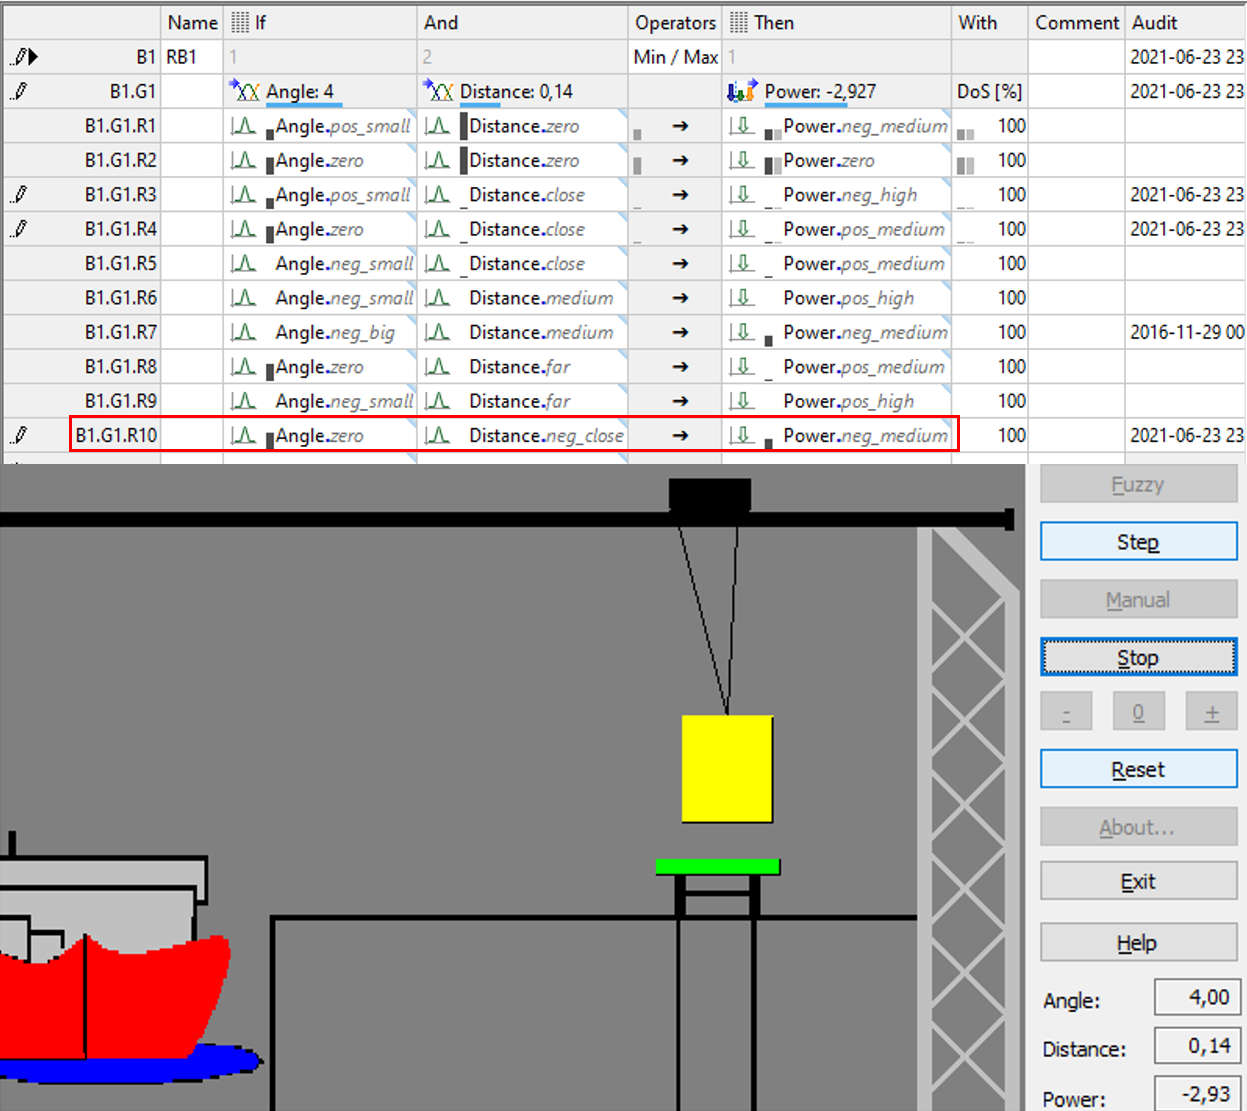
\includegraphics[width=0.7\linewidth]{Imagens/QR1/novaRegra1}
	\caption{Adição de nova regra}
	\label{fig:novaregra1}
\end{figure}

Nota-se que, com a adição dessa nova regra, a posição final do guindaste está muito próxima do ideal, com distância de $0.14$, sendo o ideal $0$.


\subsection{QR 2 - Exibindo estado inicial}

Assim como na seção anterior, a figura abaixo exibe as regras originais e a posição final original do guindaste.
\begin{figure}[H]
	\centering
	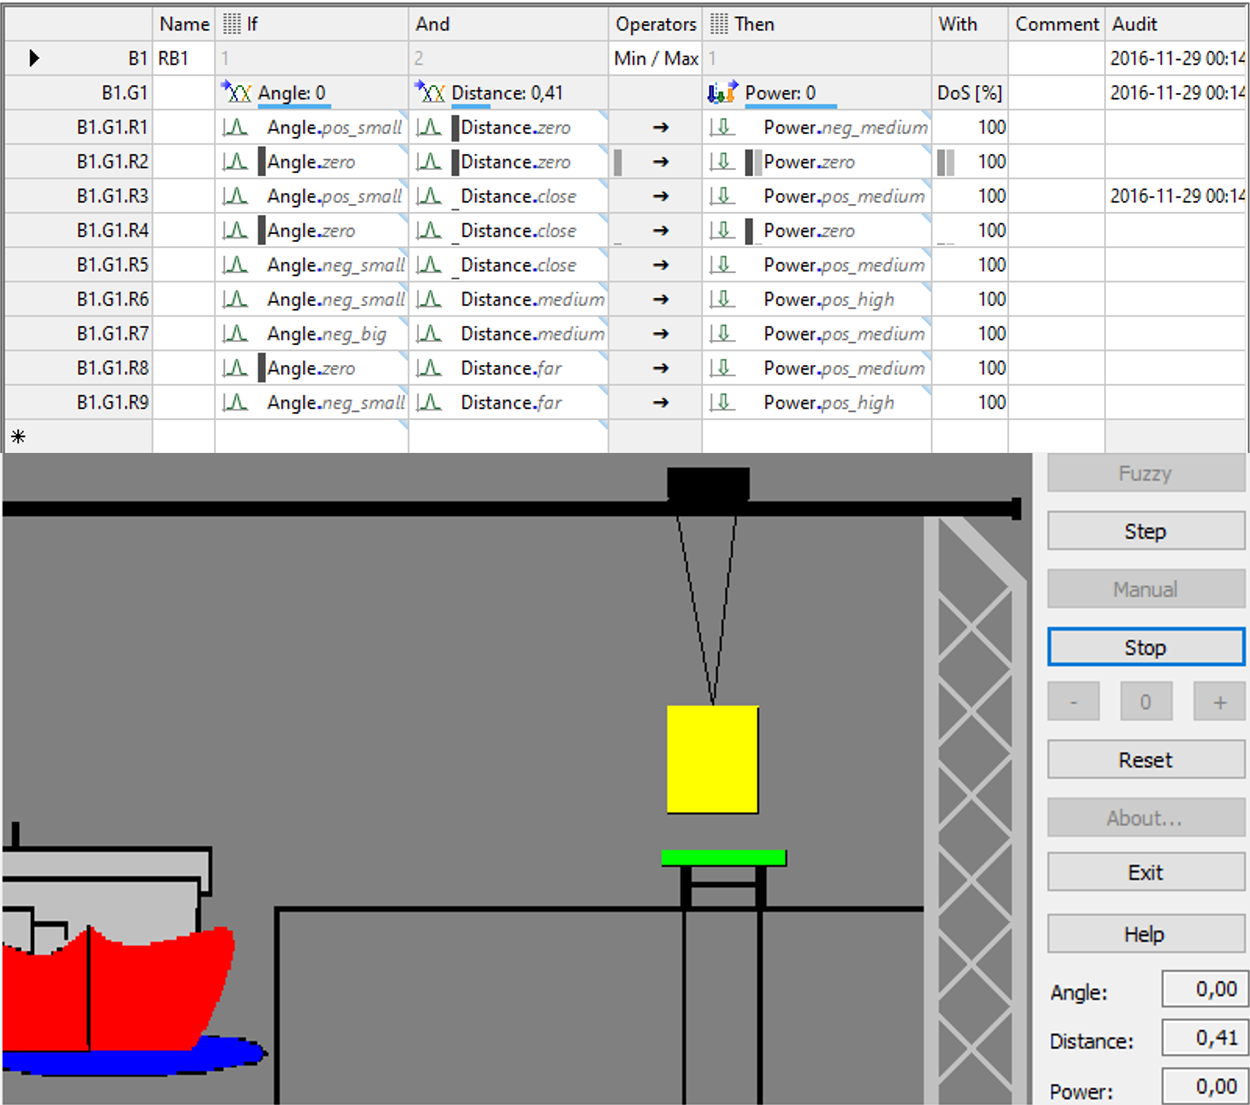
\includegraphics[width=0.7\linewidth]{Imagens/QR2/estadoOriginal}
	\caption{Regras originais e posição final original do guindaste}
	\label{fig:estadooriginal}
\end{figure}

Como pode ser percebido pelo canto inferior direito da figura \ref{fig:estadooriginal}, a posição final do guindaste está muito próxima da ideal. Dito isso, os ajustes que devem ser feitos nas regras devem estar mais relacionados com ajustes finos e finais, isto é, ajustes das regras que envolvem a variável \textit{Angle} em seus valores \textit{zero}, \textit{neg\_small} e \textit{pos\_small} e a variável \textit{Distance} em seus valores \textit{zero}, \textit{close} e \textit{neg\_close}. Além disso, a alteração nas regras deve fazer o guindaste andar um pouco mais para a direita.

\subsection{QR 2 - Alteração de Regras}

A primeira alteração a ser feita é trocar a regra $(6)$ pela regra $(7)$ abaixo.

\begin{align}
	Angle.neg\_small\&Distance.close&\to Power.pos\_medium\\
	Angle.neg\_small\&Distance.close&\to Power.neg\_medium
\end{align}

O que se espera com essa alteração é, quando o guindaste estiver muito próximo ao local desejado e com ângulo pequeno negativo, isto é, um pouco à direita do local desejado, ao invés de colocar potência positiva, que empurraria o guindaste mais para a direita, colocar potência negativa para trazê-lo um pouco mais para a esquerda. O resultado dessa alteração está exibido na figura abaixo.
\begin{figure}[H]
	\centering
	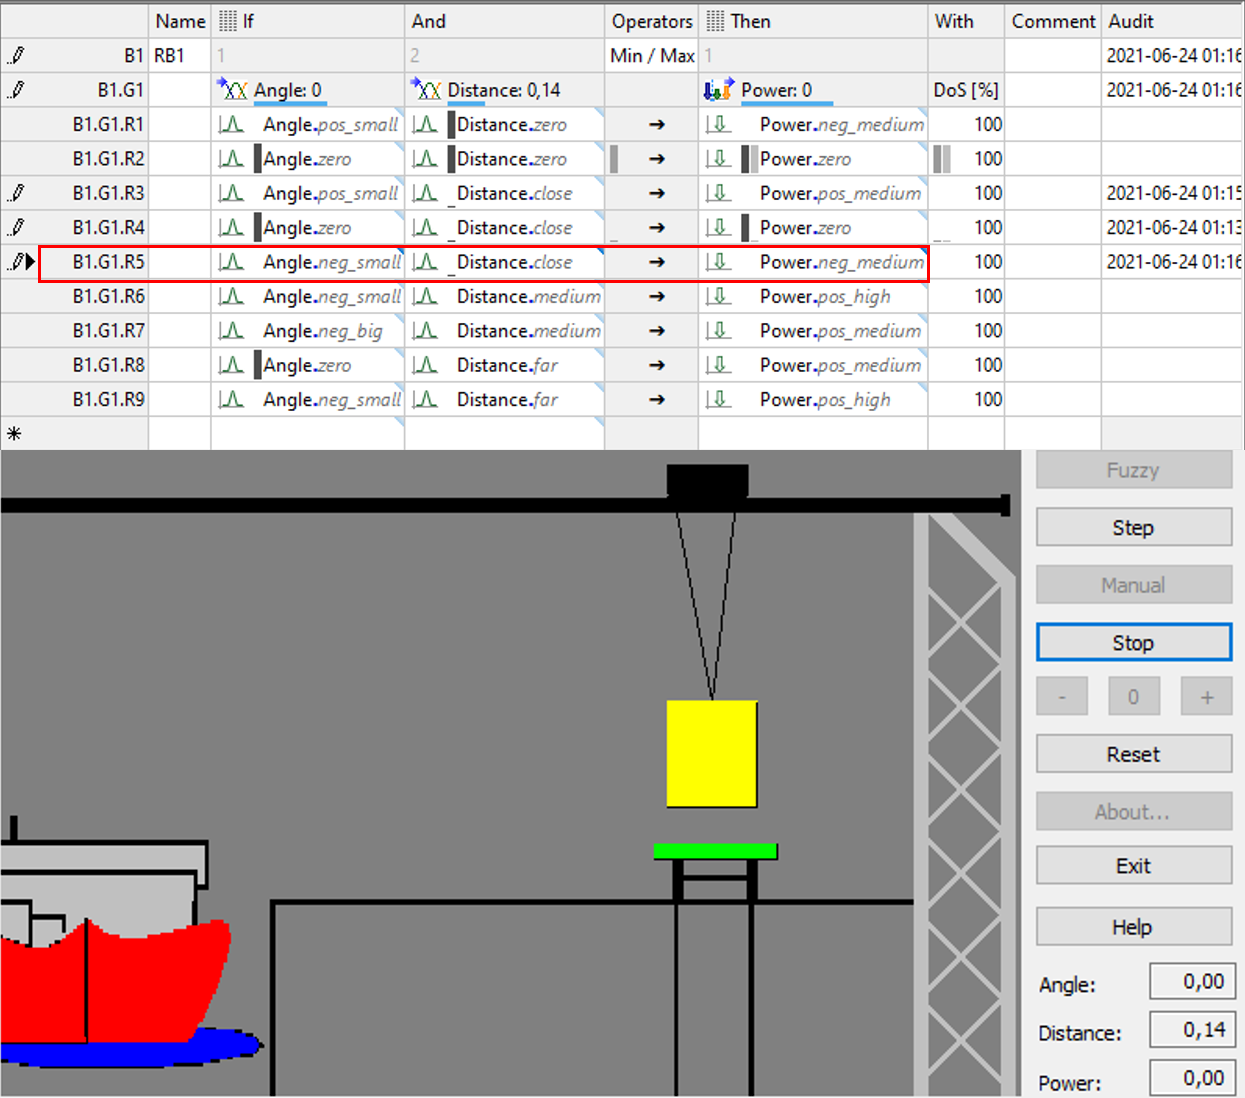
\includegraphics[width=0.8\linewidth]{Imagens/QR2/alteracao1}
	\caption{Alteração 1}
	\label{fig:alteracao1qr2}
\end{figure}

Como pode ser visto, a distância final está mais próxima da desejada, uma vez que o valor exibido caiu de $0.41$ para $0.14$, enquanto que o ângulo permaneceu em zero.

\section{Parte 2 - Problema Financiamento Imobiliário}

\subsection{Comentários Iniciais}

Primeiramente, o valor das variáveis para a minha matrícula, 1810764, são:
\begin{itemize}
	\item vl\_Localização = 50
	\item vl\_nivel\_Receita = 50
	\item vl\_Padrao\_Obra = 71
	\item vl\_Patrimonio = 58
	\item vl\_taxa\_Juros = 50	
\end{itemize}

O sistema de inferência fuzzy a ser criado segue o que está descrito no material disponibilizado na plataforma EAD e o que foi mostrado em aula. Sendo assim, podemos definir esse sistema de inferência assim como mostra a figura abaixo.
\begin{figure}[H]
	\centering
	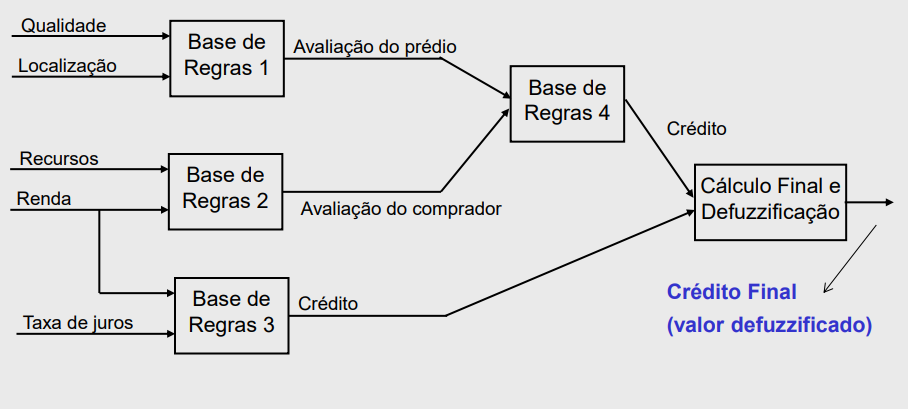
\includegraphics[width=0.9\linewidth]{Imagens/financiamento/esquemaSIF}
	\caption{Esquema do sistema de inferêcia fuzzy implementado}
	\label{fig:esquemasif}
\end{figure}

As variáveis de entrada \textit{vl\_Localização} e \textit{vl\_Padrao\_Obra} são usadas para definir a variável intermediária \textit{aval\_predio}, cuja base de dados pode ser a base 1 da figura \ref{fig:esquemasif}. As variáveis \textit{vl\_nivel\_Receita} e \textit{vl\_Patrimonio}, por sua vez, são usadas para definir a variável intermediária \textit{aval\_comprador} por meio de base de regras 2. Por fim, as variáveis \textit{vl\_taxa\_Juros} e \textit{vl\_Patrimonio} são usadas, via base de regras 3, para definir já a variável de saída \textit{credito\_fornecido}. As variáveis intermediárias \textit{aval\_predio} e \textit{aval\_comprador} são usadas, via base de regras 4, para definir a variável de saída, \textit{credito\_fornecido}.

\subsection{Montando o Sistema de Inferência Fuzzy}

\subsection{Respostas Manuais}

\subsection{Respostas FuzzyTech}

\end{document}